\documentclass[11pt,letterpaper]{article}

\usepackage[margin=1in]{geometry}
\usepackage{amsmath,amssymb}
\usepackage{graphicx}
\usepackage{booktabs}
\usepackage{array}
\usepackage{xcolor}
\usepackage{listings}
\usepackage{tikz}
\usetikzlibrary{positioning,arrows.meta,fit,backgrounds,calc}
\usepackage{hyperref}
\usepackage{enumitem}
\usepackage{fancyvrb}
\usepackage{caption}

% Colors
\definecolor{cpuBlue}{HTML}{2563EB}
\definecolor{wseColor}{HTML}{0891B2}
\definecolor{confirmGreen}{HTML}{059669}
\definecolor{conflictRed}{HTML}{DC2626}
\definecolor{warnOrange}{HTML}{D97706}
\definecolor{codeBg}{HTML}{F3F4F6}
\definecolor{codeFrame}{HTML}{D1D5DB}

% Listings style
\lstset{
  basicstyle=\ttfamily\small,
  backgroundcolor=\color{codeBg},
  frame=single,
  rulecolor=\color{codeFrame},
  breaklines=true,
  numbers=none,
  xleftmargin=4pt,
  xrightmargin=4pt,
  aboveskip=8pt,
  belowskip=8pt,
  columns=fullflexible,
  keepspaces=true,
}

\title{\textbf{Graph Coloring with CSR:\\Cerebras Approach}}
\author{Siddharth Banakar}
\date{}

\begin{document}
\maketitle

\tableofcontents
\newpage

%======================================================================
\section{The Example Graph}
%======================================================================

To keep things concrete, we will use the same small graph throughout this document: 8~vertices connected by 13~edges.

\begin{center}
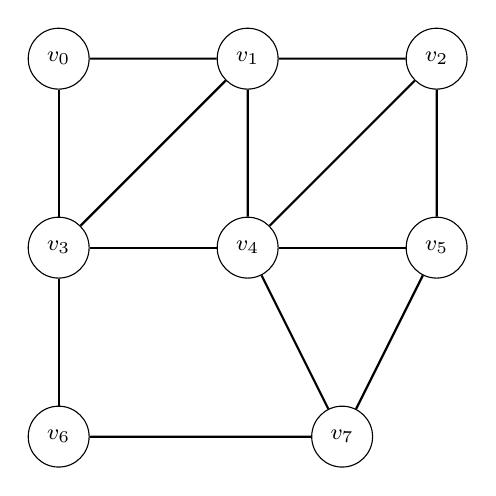
\begin{tikzpicture}[
    vertex/.style={circle, draw, minimum size=22pt, font=\footnotesize\bfseries},
    edge/.style={thick},
    scale=1.2
  ]
  % Vertices
  \node[vertex] (0) at (0,2)   {$v_0$};
  \node[vertex] (1) at (2,2)   {$v_1$};
  \node[vertex] (2) at (4,2)   {$v_2$};
  \node[vertex] (3) at (0,0)   {$v_3$};
  \node[vertex] (4) at (2,0)   {$v_4$};
  \node[vertex] (5) at (4,0)   {$v_5$};
  \node[vertex] (6) at (0,-2)  {$v_6$};
  \node[vertex] (7) at (3,-2)  {$v_7$};

  % Edges
  \draw[edge] (0)--(1); \draw[edge] (0)--(3);
  \draw[edge] (1)--(2); \draw[edge] (1)--(3); \draw[edge] (1)--(4);
  \draw[edge] (2)--(4); \draw[edge] (2)--(5);
  \draw[edge] (3)--(4); \draw[edge] (3)--(6);
  \draw[edge] (4)--(5); \draw[edge] (4)--(7);
  \draw[edge] (5)--(7); \draw[edge] (6)--(7);
\end{tikzpicture}
\end{center}

\noindent\textbf{Edge list:}
$(0,1),\;(0,3),\;(1,2),\;(1,3),\;(1,4),\;(2,4),\;(2,5),\;(3,4),\;(3,6),\;(4,5),\;(4,7),\;(5,7),\;(6,7)$

\medskip
\noindent\textbf{Degrees:}
$\deg(v_0)=2,\;\deg(v_1)=4,\;\deg(v_2)=3,\;\deg(v_3)=4,\;\deg(v_4)=5,\;\deg(v_5)=3,\;\deg(v_6)=2,\;\deg(v_7)=3$

%======================================================================
\section{Building the CSR Representation}
%======================================================================

Before we can color anything, we need a way to store the graph in memory. CSR does this with just two flat arrays:
\begin{itemize}[nosep]
  \item \texttt{offsets[$n{+}1$]}: for vertex $v$, its neighbors live at \texttt{adj[offsets[$v$]\,..\,offsets[$v{+}1$])}.
  \item \texttt{adj[$\mathit{nnz}$]}: flat array of all neighbor vertex IDs, packed contiguously.
\end{itemize}

Each undirected edge is stored as two directed arcs (both directions), so $|\texttt{adj}| = 2 \times 13 = 26$.

\begin{lstlisting}
offsets[] = [0, 2, 6, 9, 13, 18, 21, 23, 26]
             v0 v1 v2  v3   v4   v5  v6  v7  end

adj[] = [1,3 | 0,2,3,4 | 1,4,5 | 0,1,4,6 | 1,2,3,5,7 | 2,4,7 | 3,7 | 4,5,6]
         v0     v1        v2      v3         v4          v5      v6    v7
\end{lstlisting}

\paragraph{Example lookup: neighbors of $v_4$.}
\[
  \texttt{offsets}[4] = 13, \quad \texttt{offsets}[5] = 18 \quad\Longrightarrow\quad \texttt{adj}[13..18) = [1,\,2,\,3,\,5,\,7]
\]

That is all it takes to find every neighbor of a vertex: two lookups into \texttt{offsets[]} and one contiguous walk through \texttt{adj[]}. No pointer chasing, no hash tables, just simple array arithmetic.

%======================================================================
\section{CPU Sequential Coloring (Bucket Greedy)}
\label{sec:cpu}
%======================================================================

\subsection{Algorithm Overview}

Each vertex starts with a \emph{color list}, a small, randomly chosen subset of the available colors. Here is how the CPU works through them, one vertex at a time:

\begin{enumerate}[nosep]
  \item Place vertices into \textbf{buckets} by color-list size (smallest first = most constrained).
  \item Pick a vertex from the smallest non-empty bucket.
  \item Assign it a color from its list.
  \item \textbf{Propagate:} scan its CSR neighbors; remove the chosen color from each uncolored neighbor's list; move affected neighbors to smaller buckets.
  \item Repeat until all vertices are processed.
\end{enumerate}

Since we only color one vertex at a time and immediately tell its neighbors, \textbf{conflicts simply cannot happen}.

\subsection{Setup}

Let us say each vertex draws a random color list from the palette $\{C_0, C_1, C_2, C_3, C_4\}$:

\begin{center}
\begin{tabular}{ll@{\qquad}ll}
\toprule
Vertex & Color List & Vertex & Color List \\
\midrule
$v_0$ & $[C_0, C_2]$       & $v_4$ & $[C_0, C_1, C_3]$ \\
$v_1$ & $[C_1, C_2, C_3]$  & $v_5$ & $[C_0, C_2]$ \\
$v_2$ & $[C_0, C_1]$       & $v_6$ & $[C_1, C_3]$ \\
$v_3$ & $[C_0, C_2, C_3]$  & $v_7$ & $[C_0, C_1, C_2]$ \\
\bottomrule
\end{tabular}
\end{center}

\noindent\textbf{Initial buckets:}
\begin{itemize}[nosep]
  \item Bucket[2]: $v_0, v_2, v_5, v_6$ \quad(2 colors each, most constrained)
  \item Bucket[3]: $v_1, v_3, v_4, v_7$ \quad(3 colors each)
\end{itemize}

\subsection{Iteration-by-Iteration Walkthrough}

%--- Iteration 1 ---
\paragraph{Iteration 1---Pick $v_0$ from Bucket[2].}
\begin{itemize}[nosep]
  \item $v_0$ picks $C_0$ from its list $[C_0, C_2]$.
  \item Scan CSR: $\texttt{offsets}[0]=0,\;\texttt{offsets}[1]=2 \;\Rightarrow\; \texttt{adj}[0..2) = [v_1, v_3]$.
  \item $v_1$: list $[C_1,C_2,C_3]$, $C_0$ not present $\rightarrow$ skip.
  \item $v_3$: list $[C_0,C_2,C_3]$, $C_0$ found $\rightarrow$ remove $\rightarrow$ $[C_2,C_3]$.
  \item \textbf{Result:} $v_0 = C_0$.\quad $v_3$ moves Bucket[3]$\to$Bucket[2].
\end{itemize}

%--- Iteration 2 ---
\paragraph{Iteration 2---Pick $v_2$ from Bucket[2].}
\begin{itemize}[nosep]
  \item $v_2$ picks $C_1$ from list $[C_0, C_1]$.
  \item CSR neighbors: $\texttt{adj}[6..9) = [v_1, v_4, v_5]$.
  \item $v_1$: $[C_1,C_2,C_3]$, $C_1$ found $\rightarrow$ remove $\rightarrow$ $[C_2,C_3]$.
  \item $v_4$: $[C_0,C_1,C_3]$, $C_1$ found $\rightarrow$ remove $\rightarrow$ $[C_0,C_3]$.
  \item $v_5$: $[C_0,C_2]$, $C_1$ not present $\rightarrow$ skip.
  \item \textbf{Result:} $v_2 = C_1$.\quad $v_1$: Bucket[3]$\to$Bucket[2].\quad $v_4$: Bucket[3]$\to$Bucket[2].
\end{itemize}

%--- Iteration 3 ---
\paragraph{Iteration 3---Pick $v_5$ from Bucket[2].}
\begin{itemize}[nosep]
  \item $v_5$ picks $C_2$ from list $[C_0, C_2]$.
  \item CSR neighbors: $\texttt{adj}[18..21) = [v_2, v_4, v_7]$.
  \item $v_2$: already colored $\rightarrow$ skip.
  \item $v_4$: $[C_0,C_3]$, $C_2$ not present $\rightarrow$ skip.
  \item $v_7$: $[C_0,C_1,C_2]$, $C_2$ found $\rightarrow$ remove $\rightarrow$ $[C_0,C_1]$.
  \item \textbf{Result:} $v_5 = C_2$.\quad $v_7$: Bucket[3]$\to$Bucket[2].
\end{itemize}

%--- Iteration 4 ---
\paragraph{Iteration 4---Pick $v_6$ from Bucket[2].}
\begin{itemize}[nosep]
  \item $v_6$ picks $C_1$ from list $[C_1, C_3]$.
  \item CSR neighbors: $\texttt{adj}[21..23) = [v_3, v_7]$.
  \item $v_3$: $[C_2,C_3]$, $C_1$ not present $\rightarrow$ skip.
  \item $v_7$: $[C_0,C_1]$, $C_1$ found $\rightarrow$ remove $\rightarrow$ $[C_0]$.
  \item \textbf{Result:} $v_6 = C_1$.\quad $v_7$: Bucket[2]$\to$\textbf{Bucket[1]} (only 1 color left).
\end{itemize}

%--- Iteration 5 ---
\paragraph{Iteration 5---Pick $v_7$ from Bucket[1].}
\begin{itemize}[nosep]
  \item $v_7$ has only $[C_0]$, forced choice.
  \item CSR neighbors: $\texttt{adj}[23..26) = [v_4, v_5, v_6]$.
  \item $v_4$: $[C_0,C_3]$, $C_0$ found $\rightarrow$ remove $\rightarrow$ $[C_3]$.
  \item $v_5$, $v_6$: already colored $\rightarrow$ skip.
  \item \textbf{Result:} $v_7 = C_0$.\quad $v_4$: Bucket[2]$\to$Bucket[1].
\end{itemize}

%--- Iteration 6 ---
\paragraph{Iteration 6---Pick $v_4$ from Bucket[1].}
\begin{itemize}[nosep]
  \item $v_4$ has only $[C_3]$, forced choice.
  \item CSR neighbors: $\texttt{adj}[13..18) = [v_1, v_2, v_3, v_5, v_7]$.
  \item $v_1$: $[C_2,C_3]$, $C_3$ found $\rightarrow$ remove $\rightarrow$ $[C_2]$.
  \item $v_3$: $[C_2,C_3]$, $C_3$ found $\rightarrow$ remove $\rightarrow$ $[C_2]$.
  \item $v_2, v_5, v_7$: already colored $\rightarrow$ skip.
  \item \textbf{Result:} $v_4 = C_3$.\quad $v_1,v_3$: Bucket[2]$\to$Bucket[1].
\end{itemize}

%--- Iterations 7-8 ---
\paragraph{Iterations 7--8---$v_1$ and $v_3$ (both forced).}
\begin{itemize}[nosep]
  \item $v_1$ has only $[C_2]$ $\rightarrow$ $v_1 = C_2$.
  \item $v_3$ has only $[C_2]$ $\rightarrow$ $v_3 = C_2$.
\end{itemize}

\subsection{Final CPU Result}

\begin{center}
\fbox{$v_0{=}C_0 \quad v_1{=}C_2 \quad v_2{=}C_1 \quad v_3{=}C_2 \quad v_4{=}C_3 \quad v_5{=}C_2 \quad v_6{=}C_1 \quad v_7{=}C_0$}
\end{center}

\noindent\textbf{8 sequential iterations, 4 colors used, 0 conflicts.}

\subsection{Why It Works}

Notice how every iteration follows the same simple recipe:
\begin{enumerate}[nosep]
  \item Look up \texttt{offsets[$v$]} and \texttt{offsets[$v{+}1$]} to find where this vertex's neighbors live in \texttt{adj[]}.
  \item Walk through that contiguous slice to visit each neighbor.
  \item If a neighbor has not been colored yet and the chosen color appears in its list, cross it off.
\end{enumerate}

Because we propagate the color choice right away, no two neighbors can ever accidentally end up wearing the same color. The price we pay: \textbf{we can only color one vertex per step}, making the whole process strictly sequential.

%======================================================================
\section{Cerebras WSE Speculative Parallel Coloring}
\label{sec:cerebras}
%======================================================================

\subsection{Algorithm Overview}

The 8 vertices are \textbf{distributed across 4 Processing Elements (PEs)}, 2~vertices each:

\begin{center}
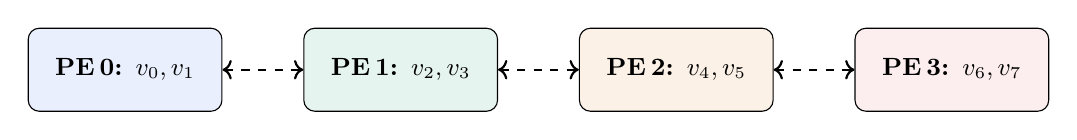
\begin{tikzpicture}[
    pe/.style={draw, rounded corners=4pt, minimum width=70pt, minimum height=30pt, font=\small\bfseries},
  ]
  \node[pe, fill=cpuBlue!10]  (pe0) at (0,0)   {PE\,0: $v_0, v_1$};
  \node[pe, fill=confirmGreen!10] (pe1) at (3.5,0) {PE\,1: $v_2, v_3$};
  \node[pe, fill=warnOrange!10]   (pe2) at (7,0)   {PE\,2: $v_4, v_5$};
  \node[pe, fill=conflictRed!8]   (pe3) at (10.5,0) {PE\,3: $v_6, v_7$};
  \draw[<->,thick,dashed] (pe0)--(pe1);
  \draw[<->,thick,dashed] (pe1)--(pe2);
  \draw[<->,thick,dashed] (pe2)--(pe3);
\end{tikzpicture}
\end{center}

Each PE holds its own slice of the CSR in local SRAM. The key difference from the CPU: all PEs work \textbf{at the same time}:
\begin{enumerate}[nosep]
  \item Every PE picks \emph{tentative} colors for its uncolored vertices, without waiting for anyone else.
  \item Each PE checks edges within its own partition for obvious clashes.
  \item PEs then \textbf{exchange} their boundary colors with neighbors via tiny hardware messages called \emph{wavelets}.
  \item Each PE looks at the incoming messages and flags any conflicts on cross-PE edges.
  \item Conflicts are resolved with a dead-simple rule: \textbf{the vertex with the higher ID backs off} and tries again next round.
  \item Repeat until every vertex has a confirmed color.
\end{enumerate}

\subsection{Setup}

We start with the same color lists as the CPU example, so we can compare apples to apples:

\begin{center}
\begin{tabular}{lll}
\toprule
PE & Vertex & Color List \\
\midrule
PE\,0 & $v_0$ & $[C_0, C_2]$ \\
PE\,0 & $v_1$ & $[C_1, C_2, C_3]$ \\
\midrule
PE\,1 & $v_2$ & $[C_0, C_1]$ \\
PE\,1 & $v_3$ & $[C_0, C_2, C_3]$ \\
\midrule
PE\,2 & $v_4$ & $[C_0, C_1, C_3]$ \\
PE\,2 & $v_5$ & $[C_0, C_2]$ \\
\midrule
PE\,3 & $v_6$ & $[C_1, C_3]$ \\
PE\,3 & $v_7$ & $[C_0, C_1, C_2]$ \\
\bottomrule
\end{tabular}
\end{center}

\subsection{Round 1}

\paragraph{Step 1: Speculate.}
All four PEs grab a tentative color at the same instant. Nobody waits for anyone else:

\begin{center}
\begin{tabular}{llll}
PE\,0: & $v_0 \to C_0$ & $v_1 \to C_1$ & \\
PE\,1: & $v_2 \to C_0$ & $v_3 \to C_0$ & \\
PE\,2: & $v_4 \to C_0$ & $v_5 \to C_0$ & \\
PE\,3: & $v_6 \to C_1$ & $v_7 \to C_0$ & \\
\end{tabular}
\end{center}

\paragraph{Step 2: Local check (within each PE).}
\begin{itemize}[nosep]
  \item PE\,0: edge $(v_0,v_1)$: $C_0 \neq C_1$, no conflict.
  \item PE\,1: no edge between $v_2,v_3$, no conflict.
  \item PE\,2: edge $(v_4,v_5)$: $C_0 = C_0$, \textcolor{conflictRed}{\textbf{LOCAL CONFLICT!}} $v_5$ yields (ID\,$5 > 4$).
  \item PE\,3: edge $(v_6,v_7)$: $C_1 \neq C_0$, no conflict.
\end{itemize}

\paragraph{Step 3: Wavelet exchange.}
Each PE sends its boundary vertex colors to neighboring PEs:
\begin{itemize}[nosep]
  \item PE\,0 sends $v_0{=}C_0,\; v_1{=}C_1$ to PE\,1, PE\,2.
  \item PE\,1 sends $v_2{=}C_0,\; v_3{=}C_0$ to PE\,0, PE\,2.
  \item PE\,2 sends $v_4{=}C_0,\; v_5{=}\text{uncolored}$ to PE\,0, PE\,1, PE\,3.
  \item PE\,3 sends $v_6{=}C_1,\; v_7{=}C_0$ to PE\,2.
\end{itemize}

\paragraph{Step 4: Detect boundary conflicts.}
\begin{center}
\begin{tabular}{lccl}
\toprule
Edge & Colors & Match? & Resolution \\
\midrule
$(v_0,v_3)$ & $C_0 = C_0$ & \textcolor{conflictRed}{\textbf{Yes}} & $v_3$ yields (ID\,$3>0$) \\
$(v_1,v_3)$ & $C_1 \neq C_0$ & \textcolor{confirmGreen}{No} & N/A \\
$(v_1,v_4)$ & $C_1 \neq C_0$ & \textcolor{confirmGreen}{No} & N/A \\
$(v_2,v_4)$ & $C_0 = C_0$ & \textcolor{conflictRed}{\textbf{Yes}} & $v_4$ yields (ID\,$4>2$) \\
$(v_6,v_7)$ & $C_1 \neq C_0$ & \textcolor{confirmGreen}{No} & N/A \\
\bottomrule
\end{tabular}
\end{center}

\paragraph{Round 1 result.}
\begin{itemize}[nosep]
  \item \textcolor{confirmGreen}{\textbf{Confirmed (5):}} $v_0{=}C_0,\; v_1{=}C_1,\; v_2{=}C_0,\; v_6{=}C_1,\; v_7{=}C_0$.
  \item \textcolor{conflictRed}{\textbf{Yielded (3):}} $v_3,\; v_4,\; v_5$ revert to uncolored for next round.
\end{itemize}

\medskip
\noindent\emph{In one parallel round we colored 5 out of 8 vertices. The CPU needed 5 separate sequential steps to get this far.}

\subsection{Round 2}

\paragraph{Step 1: Speculate (only uncolored vertices).}
Each vertex avoids colors already confirmed by its neighbors:
\begin{itemize}[nosep]
  \item $v_3$: neighbors $v_0{=}C_0, v_1{=}C_1$ $\Rightarrow$ avoid $\{C_0,C_1\}$ $\Rightarrow$ picks $C_2$.
  \item $v_4$: neighbors $v_1{=}C_1, v_2{=}C_0, v_7{=}C_0$ $\Rightarrow$ avoid $\{C_0,C_1\}$ $\Rightarrow$ picks $C_3$.
  \item $v_5$: neighbors $v_2{=}C_0, v_7{=}C_0$ $\Rightarrow$ avoid $\{C_0\}$ $\Rightarrow$ picks $C_2$.
\end{itemize}

\paragraph{Step 2: Local check.}
\begin{itemize}[nosep]
  \item PE\,1: $v_3{=}C_2$ (only uncolored vertex on this PE) $\rightarrow$ no local conflict.
  \item PE\,2: edge $(v_4,v_5)$: $C_3 \neq C_2$, no conflict.
\end{itemize}

\paragraph{Step 3--4: Wavelet exchange + boundary check.}
\begin{center}
\begin{tabular}{lccl}
\toprule
Edge & Colors & Match? \\
\midrule
$(v_3,v_4)$ & $C_2 \neq C_3$ & \textcolor{confirmGreen}{No} \\
$(v_3,v_6)$ & $C_2 \neq C_1$ & \textcolor{confirmGreen}{No} \\
$(v_5,v_7)$ & $C_2 \neq C_0$ & \textcolor{confirmGreen}{No} \\
\bottomrule
\end{tabular}
\end{center}

\noindent\textbf{No conflicts.} All three vertices confirmed.

\subsection{Final Cerebras Result}

\begin{center}
\fbox{$v_0{=}C_0 \quad v_1{=}C_1 \quad v_2{=}C_0 \quad v_3{=}C_2 \quad v_4{=}C_3 \quad v_5{=}C_2 \quad v_6{=}C_1 \quad v_7{=}C_0$}
\end{center}

\noindent\textbf{2 parallel rounds, 4 colors used, 3 conflicts resolved in round~1.}

%======================================================================
\section{Deep Dive: How Wavelet Exchange Works}
\label{sec:wavelets}
%======================================================================

A natural question comes up: once every PE has picked its tentative colors, \emph{how does it find out what colors the other PEs chose?} After all, each PE can only see its own vertices. The answer is \textbf{wavelet exchange}, a lightweight, hardware-routed messaging system built directly into the WSE fabric.

\subsection{The Problem}

Right after speculation, every PE is in the dark. It knows the colors it assigned to \textbf{its own} vertices, but has \textbf{absolutely no clue} what colors the other PEs chose. The local CSR tells it \emph{who} the remote neighbors are, but says nothing about what color they just picked.

\subsection{Three Phases of Communication}

\paragraph{Phase 1---Speculate (purely local).}
Every PE picks tentative colors on its own. No messages fly yet.

\paragraph{Phase 2---Send wavelets.}
Now each PE walks through its local CSR looking for \textbf{boundary edges}, i.e., edges where one endpoint belongs to a different PE. For every such edge, it fires off a small message (a \emph{wavelet}) through the hardware fabric:

\begin{center}
\texttt{wavelet = \{ vertex\_id, color\_assigned \}}
\end{center}

For example, PE\,0 looks at $v_0$'s neighbors in the CSR: $[v_1, v_3]$.
\begin{itemize}[nosep]
  \item $v_1$ is local (on PE\,0) $\rightarrow$ no wavelet needed, check directly.
  \item $v_3$ is on PE\,1 $\rightarrow$ \textbf{send wavelet} \texttt{(v0, C0)} to PE\,1.
\end{itemize}

Similarly, PE\,1 sends \texttt{(v3, C0)} to PE\,0 (for edge $v_3 \leftrightarrow v_0$), and \texttt{(v3, C0)} to PE\,2 (for edge $v_3 \leftrightarrow v_4$), etc.

On the WSE hardware, wavelets travel through the \textbf{2D mesh fabric}, a physical network connecting all 750,000+ PEs. Each wavelet is a small data packet routed along the grid. This takes only a few clock cycles, not a network round-trip.

\paragraph{Phase 3---Receive and detect.}
When PE\,1 gets the wavelet \texttt{(v0, C0)}, it immediately checks: ``My vertex $v_3$ is a neighbor of $v_0$, and I gave $v_3$ the color $C_0$ too. That is a \textbf{conflict!}'' Since $3 > 0$, $v_3$ is the one that backs off and reverts to uncolored.

\subsection{Why This Is Fast}

\begin{center}
\renewcommand{\arraystretch}{1.3}
\begin{tabular}{>{\raggedright}p{3.4cm} p{9cm}}
\toprule
\textbf{Aspect} & \textbf{Detail} \\
\midrule
Wavelet size & Just a \texttt{(vertex\_id, color)} pair, a few bytes \\
Transport & Hardware-routed on the wafer's 2D mesh, not software networking \\
Latency & Single-digit clock cycles between adjacent PEs \\
Parallelism & All PEs send and receive wavelets \textbf{simultaneously} \\
\bottomrule
\end{tabular}
\end{center}

The whole speculate $\to$ exchange $\to$ detect $\to$ resolve cycle makes up a single ``round,'' and every PE on the wafer runs through it at the same time.

%======================================================================
\section{Why Conflicts Never Cascade: Deterministic Resolution}
\label{sec:resolution}
%======================================================================

\subsection{The Rule: Higher ID Always Yields}

The rule is almost trivially simple. Whenever two neighboring vertices end up with the same color and $i < j$:
\begin{itemize}[nosep]
  \item $v_i$ (the lower ID) \textbf{keeps} its color.
  \item $v_j$ (the higher ID) \textbf{gives up} and goes back to uncolored for the next round
\end{itemize}

The beauty of this rule is that both PEs can apply it \textbf{independently}. Neither one has to ask the other what to do.

\subsection{Why ``Both Yield'' or ``Both Keep'' Is Impossible}

Consider edge $(v_0, v_3)$ with $C_0 = C_0$:

\begin{center}
\renewcommand{\arraystretch}{1.3}
\begin{tabular}{lll}
\toprule
\textbf{PE} & \textbf{Sees} & \textbf{Decides} \\
\midrule
PE\,0 & ``My $v_0$ conflicts with $v_3$. Since $0 < 3$, \textbf{I win}.'' & Keeps $v_0 = C_0$ \\
PE\,1 & ``My $v_3$ conflicts with $v_0$. Since $3 > 0$, \textbf{I yield}.'' & Reverts $v_3$ \\
\bottomrule
\end{tabular}
\end{center}

This works because vertex IDs form a \textbf{total order}: for any two vertices, one ID is always strictly smaller than the other. There are no ties (every ID is unique), no coin flips, and no back-and-forth negotiation. Both PEs look at the same two numbers and always reach the same conclusion.

\subsection{What About the Next Round?}

After yielding, $v_3$ tries a \textbf{new} color in round~2 (say $C_2$). Could it clash with $v_0{=}C_0$ again? \textbf{No}, because $v_0$ is already locked in, and $v_3$ remembers from the wavelet it received that $v_0$ took $C_0$, so it steers clear.

But could $v_3$ run into a \emph{different} neighbor that also just grabbed $C_2$? \textbf{Yes}, and if that happens, the same higher-ID-yields rule kicks in again. The point is that every round clears out all current conflicts, and the pool of uncolored vertices keeps shrinking. On average, about half the conflicting vertices survive each round, which is why the total number of rounds grows only as $O(\log n)$.

%======================================================================
\section{Worst Case: All PEs in Conflict}
\label{sec:worstcase}
%======================================================================

To really put the conflict-resolution rule through its paces, let us construct a nightmare scenario where \textbf{every single PE pair} ends up with a cross-PE conflict in Round~1.

\subsection{Setup}

Suppose every vertex speculatively picks one of just two colors:

\begin{center}
\begin{tabular}{llll}
\toprule
PE & Vertex & Tentative & PE & Vertex & Tentative \\
\midrule
PE\,0 & $v_0$ & $C_0$ & PE\,2 & $v_4$ & $C_0$ \\
PE\,0 & $v_1$ & $C_1$ & PE\,2 & $v_5$ & $C_1$ \\
PE\,1 & $v_2$ & $C_1$ & PE\,3 & $v_6$ & $C_0$ \\
PE\,1 & $v_3$ & $C_0$ & PE\,3 & $v_7$ & $C_1$ \\
\bottomrule
\end{tabular}
\end{center}

\subsection{Six Boundary Conflicts Detected}

After wavelet exchange, every PE pair is involved in at least one conflict:

\begin{center}
\renewcommand{\arraystretch}{1.2}
\begin{tabular}{lcccl}
\toprule
Edge & PEs & Colors & Conflict? & Resolution \\
\midrule
$(v_0,v_3)$ & PE\,0 $\leftrightarrow$ PE\,1 & $C_0 = C_0$ & \textcolor{conflictRed}{\textbf{Yes}} & $v_3$ yields ($3>0$) \\
$(v_1,v_2)$ & PE\,0 $\leftrightarrow$ PE\,1 & $C_1 = C_1$ & \textcolor{conflictRed}{\textbf{Yes}} & $v_2$ yields ($2>1$) \\
$(v_2,v_5)$ & PE\,1 $\leftrightarrow$ PE\,2 & $C_1 = C_1$ & \textcolor{conflictRed}{\textbf{Yes}} & $v_5$ yields ($5>2$) \\
$(v_3,v_4)$ & PE\,1 $\leftrightarrow$ PE\,2 & $C_0 = C_0$ & \textcolor{conflictRed}{\textbf{Yes}} & $v_4$ yields ($4>3$) \\
$(v_3,v_6)$ & PE\,1 $\leftrightarrow$ PE\,3 & $C_0 = C_0$ & \textcolor{conflictRed}{\textbf{Yes}} & $v_6$ yields ($6>3$) \\
$(v_5,v_7)$ & PE\,2 $\leftrightarrow$ PE\,3 & $C_1 = C_1$ & \textcolor{conflictRed}{\textbf{Yes}} & $v_7$ yields ($7>5$) \\
\bottomrule
\end{tabular}
\end{center}

\subsection{Each PE Resolves Independently}

Here is the key: no PE needs to talk to any other PE \emph{about what to do}. Each one just looks at the vertex IDs and makes the call on its own:

\begin{center}
\renewcommand{\arraystretch}{1.2}
\begin{tabular}{llcl}
\toprule
PE & Vertex & Conflicts With & Decision \\
\midrule
PE\,0 & $v_0$ & $v_3$ ($0<3$) & \textcolor{confirmGreen}{\textbf{Keeps} $C_0$} \\
PE\,0 & $v_1$ & $v_2$ ($1<2$) & \textcolor{confirmGreen}{\textbf{Keeps} $C_1$} \\
PE\,1 & $v_2$ & $v_1$ ($2>1$) & \textcolor{conflictRed}{\textbf{Yields}} \\
PE\,1 & $v_3$ & $v_0$ ($3>0$) & \textcolor{conflictRed}{\textbf{Yields}} \\
PE\,2 & $v_4$ & $v_3$ ($4>3$) & \textcolor{conflictRed}{\textbf{Yields}} \\
PE\,2 & $v_5$ & $v_2$ ($5>2$) & \textcolor{conflictRed}{\textbf{Yields}} \\
PE\,3 & $v_6$ & $v_3$ ($6>3$) & \textcolor{conflictRed}{\textbf{Yields}} \\
PE\,3 & $v_7$ & $v_5$ ($7>5$) & \textcolor{conflictRed}{\textbf{Yields}} \\
\bottomrule
\end{tabular}
\end{center}

\noindent\textbf{Result:} Only $v_0{=}C_0$ and $v_1{=}C_1$ are confirmed; 6~vertices yield.

\subsection{A Vertex Can Be in Multiple Conflicts}

$v_3$ participates in \textbf{three} conflicting edges:

\begin{center}
\begin{tabular}{lcl}
\toprule
Edge & $v_3$'s Role & Outcome \\
\midrule
$(v_0,v_3)$ & Higher ID $\rightarrow$ \textbf{yields} & $v_3$ loses \\
$(v_3,v_4)$ & Lower ID $\rightarrow$ would keep & (irrelevant) \\
$(v_3,v_6)$ & Lower ID $\rightarrow$ would keep & (irrelevant) \\
\bottomrule
\end{tabular}
\end{center}

It only takes \textbf{one} losing conflict to knock a vertex out for the round. $v_3$ gives up because it lost to $v_0$. It does not matter that it would have beaten $v_4$ and $v_6$.

\subsection{Round 2 Recovery}

Now the 6 uncolored vertices are not starting from scratch; they remember the confirmed colors they learned from Round~1's wavelets:

\begin{center}
\renewcommand{\arraystretch}{1.2}
\begin{tabular}{llll}
\toprule
Vertex & Confirmed Neighbors & Must Avoid & Picks \\
\midrule
$v_2$ & $v_1{=}C_1$ & $\{C_1\}$ & $C_0$ \\
$v_3$ & $v_0{=}C_0,\; v_1{=}C_1$ & $\{C_0, C_1\}$ & $C_2$ \\
$v_4$ & $v_1{=}C_1$ & $\{C_1\}$ & $C_3$ \\
$v_5$ & (none) & $\{\}$ & $C_2$ \\
$v_6$ & (none) & $\{\}$ & $C_3$ \\
$v_7$ & (none) & $\{\}$ & $C_0$ \\
\bottomrule
\end{tabular}
\end{center}

\noindent\textbf{No conflicts.} All three vertices confirmed.

%======================================================================
\section{Barrier Synchronization Between Phases}
\label{sec:barrier}
%======================================================================

You might wonder: do all PEs really stay in lockstep? Yes. Each round is split into \textbf{strict phases} separated by hardware barriers. No PE is allowed to jump ahead until every other PE has finished the current phase:

\begin{center}
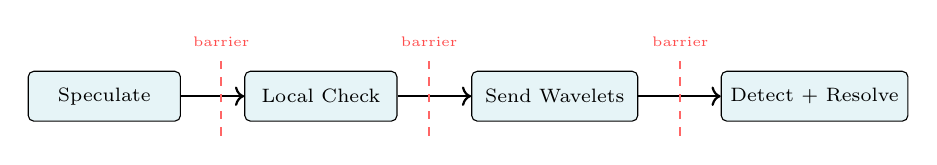
\begin{tikzpicture}[
    phase/.style={draw, rounded corners=2pt, minimum height=18pt, font=\scriptsize, fill=wseColor!10},
    barrier/.style={draw, dashed, thick, red!60},
    xscale=1.1
  ]
  \node[phase, minimum width=55pt] (s) at (0,0) {Speculate};
  \node[phase, minimum width=55pt] (l) at (2.5,0) {Local Check};
  \node[phase, minimum width=60pt] (w) at (5.2,0) {Send Wavelets};
  \node[phase, minimum width=65pt] (d) at (8.2,0) {Detect + Resolve};

  \draw[->,thick] (s)--(l);
  \draw[->,thick] (l)--(w);
  \draw[->,thick] (w)--(d);

  % Barriers
  \draw[barrier] (1.35,-0.5)--(1.35,0.5) node[above,font=\tiny,red!70] {barrier};
  \draw[barrier] (3.75,-0.5)--(3.75,0.5) node[above,font=\tiny,red!70] {barrier};
  \draw[barrier] (6.65,-0.5)--(6.65,0.5) node[above,font=\tiny,red!70] {barrier};
\end{tikzpicture}
\end{center}

\subsection{Why the Barrier After Wavelet Exchange Matters}

Imagine PE\,0 gets impatient and starts checking for conflicts \textbf{before} PE\,2 has finished sending its wavelets. PE\,0 would never see the message \texttt{``v4=C0''} and would wrongly conclude there is no conflict on edge $(v_1, v_4)$. That would be a silent bug.

\begin{quote}
\textbf{Every PE must finish sending AND receiving all wavelets before anyone starts checking for conflicts.}
\end{quote}

\subsection{How Barriers Work on the WSE}

On a regular CPU cluster, barriers are painful; they mean network round-trips, OS scheduling overhead, and wasted time. On the Cerebras WSE, the story is completely different:

\begin{center}
\renewcommand{\arraystretch}{1.3}
\begin{tabular}{>{\raggedright}p{3.2cm} p{9.5cm}}
\toprule
\textbf{Mechanism} & \textbf{How It Works} \\
\midrule
Hardware barrier & The fabric has a built-in synchronization primitive: a single signal that propagates across the wafer in a few clock cycles \\
BSP model & Cerebras uses \textbf{Bulk Synchronous Parallel}: compute, communicate, sync, repeat. It is baked into the programming model (CSL/SDK) \\
Cost & A barrier across 750,000 PEs takes ${\sim}$tens of nanoseconds, a physical wavefront on silicon, not a software message \\
\bottomrule
\end{tabular}
\end{center}

\subsection{What Happens During the Wait}

Think of it like a group of friends agreeing to wait at a checkpoint before moving on. A fast PE (say PE\,3, which only has 2 boundary edges) finishes sending almost instantly and sits idle. A busy PE (say PE\,2, with lots of boundary edges) takes a bit longer. During that gap:
\begin{itemize}[nosep]
  \item \textbf{The fast PEs just wait}, but the wait is measured in nanoseconds, not milliseconds, so it is practically free.
  \item \textbf{Nobody moves on} until the slowest PE catches up.
\end{itemize}

This is exactly why \textbf{good graph partitioning matters}: if one PE gets stuck with $10\times$ more boundary edges than the rest, everyone else twiddles their thumbs waiting for it. A balanced partition keeps the slowest PE from becoming a bottleneck.

\begin{center}
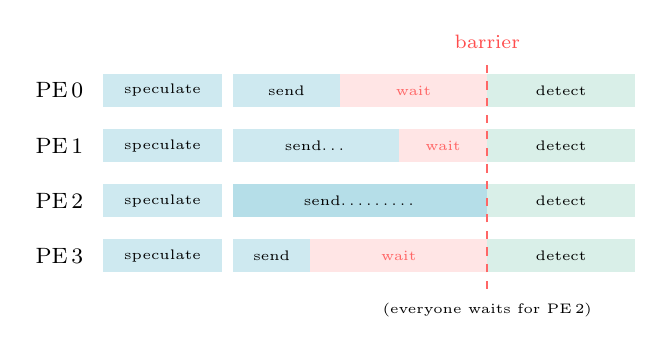
\begin{tikzpicture}[xscale=0.75, yscale=0.7]
  \footnotesize
  % Labels
  \node[anchor=east] at (-0.2, 3) {PE\,0};
  \node[anchor=east] at (-0.2, 2) {PE\,1};
  \node[anchor=east] at (-0.2, 1) {PE\,2};
  \node[anchor=east] at (-0.2, 0) {PE\,3};

  % PE 0
  \fill[wseColor!20] (0,2.7) rectangle (2,3.3); \node[font=\tiny] at (1,3) {speculate};
  \fill[wseColor!20] (2.2,2.7) rectangle (4,3.3); \node[font=\tiny] at (3.1,3) {send};
  \fill[red!10] (4,2.7) rectangle (6.5,3.3); \node[font=\tiny,red!60] at (5.25,3) {wait};
  \fill[confirmGreen!15] (6.5,2.7) rectangle (9,3.3); \node[font=\tiny] at (7.75,3) {detect};

  % PE 1
  \fill[wseColor!20] (0,1.7) rectangle (2,2.3); \node[font=\tiny] at (1,2) {speculate};
  \fill[wseColor!20] (2.2,1.7) rectangle (5,2.3); \node[font=\tiny] at (3.6,2) {send\dots};
  \fill[red!10] (5,1.7) rectangle (6.5,2.3); \node[font=\tiny,red!60] at (5.75,2) {wait};
  \fill[confirmGreen!15] (6.5,1.7) rectangle (9,2.3); \node[font=\tiny] at (7.75,2) {detect};

  % PE 2 (slowest)
  \fill[wseColor!20] (0,0.7) rectangle (2,1.3); \node[font=\tiny] at (1,1) {speculate};
  \fill[wseColor!30] (2.2,0.7) rectangle (6.5,1.3); \node[font=\tiny] at (4.35,1) {send\dots\dots\dots};
  \fill[confirmGreen!15] (6.5,0.7) rectangle (9,1.3); \node[font=\tiny] at (7.75,1) {detect};

  % PE 3
  \fill[wseColor!20] (0,-0.3) rectangle (2,0.3); \node[font=\tiny] at (1,0) {speculate};
  \fill[wseColor!20] (2.2,-0.3) rectangle (3.5,0.3); \node[font=\tiny] at (2.85,0) {send};
  \fill[red!10] (3.5,-0.3) rectangle (6.5,0.3); \node[font=\tiny,red!60] at (5,0) {wait};
  \fill[confirmGreen!15] (6.5,-0.3) rectangle (9,0.3); \node[font=\tiny] at (7.75,0) {detect};

  % Barrier line
  \draw[dashed, thick, red!60] (6.5,-0.6)--(6.5,3.6);
  \node[font=\scriptsize, red!70, anchor=south] at (6.5,3.6) {barrier};
  \node[font=\tiny, anchor=north] at (6.5,-0.7) {(everyone waits for PE\,2)};
\end{tikzpicture}
\end{center}

%======================================================================
\section{Memory Efficiency: Fitting in 48\,KB per PE}
\label{sec:memory}
%======================================================================

Here is the hard constraint that shapes everything: each PE on the WSE-2 has only \textbf{48\,KB of SRAM}. That is it: no cache, no DRAM, no disk to spill over to. The algorithm's code, all its data, and every incoming message must squeeze into that tiny budget. This is why the paper is titled ``Picasso: \textbf{Memory-Efficient} Graph Coloring.''

\subsection{The Wavelet Storage Problem}

Let us think about what PE\,2 is dealing with. It holds $v_4$, which has 5 neighbors: $v_1, v_2, v_3, v_5, v_7$. After the wavelet exchange, PE\,2 has received:

\begin{lstlisting}
From PE 0:  "v1 = C1"
From PE 1:  "v2 = C0", "v3 = C0"
From PE 3:  "v7 = C0"
(v5 is local -- no wavelet needed)
\end{lstlisting}

That is 4 incoming wavelets for just one vertex's boundary neighbors. Now imagine what happens at real-world scale:

\begin{center}
\renewcommand{\arraystretch}{1.2}
\begin{tabular}{lccc}
\toprule
\textbf{Graph Scale} & \textbf{Vertex Degree} & \textbf{Boundary Neighbors} & \textbf{Wavelets per PE} \\
\midrule
Toy (this example) & 5 & 4 & 4 \\
Real-world sparse & ${\sim}50$ & ${\sim}20$ & ${\sim}40$ \\
Dense molecular & ${\sim}500$ & ${\sim}200$ & ${\sim}400+$ \\
\bottomrule
\end{tabular}
\end{center}

\subsection{Solution 1: Process Wavelets on Arrival}

The trick is to \textbf{never actually store the wavelets}. Instead, each PE has a \emph{wavelet handler}, a tiny callback that runs the moment a wavelet shows up:

\begin{lstlisting}
// Conceptual CSL handler on each PE
on_wavelet_received(sender_vertex, sender_color):
    for each local vertex v that neighbors sender_vertex:
        if v.tentative_color == sender_color:
            v.has_conflict = true    // just set a 1-bit flag
\end{lstlisting}

The wavelet gets consumed on the spot; it never sits in a buffer eating up precious memory. All we keep per vertex is a \textbf{1-bit conflict flag}, not the full history of every message.

\subsection{Solution 2: Small Palettes by Design}

Picasso also keeps palettes intentionally small. Each vertex gets roughly $\deg(v) / \log(n)$ colors, not the full rainbow. This keeps per-vertex storage very lean:

\begin{lstlisting}
Per vertex storage:
  color           (1 int)         =  4 bytes
  has_conflict    (1 bit)         =  1 byte
  color_list      (~5 entries)    = 20 bytes
  CSR offset slice                = varies
\end{lstlisting}

\subsection{Solution 3: CSR Is the Tightest Packing}

\begin{center}
\renewcommand{\arraystretch}{1.2}
\begin{tabular}{>{\raggedright}p{4cm} p{8.5cm}}
\toprule
\textbf{Representation} & \textbf{Memory for 100 local vertices, avg degree 50} \\
\midrule
Adjacency matrix & $100 \times N_{\text{total}}$ bits, \textbf{doesn't fit} \\
Adjacency list (pointers) & 100 pointers + 5000 entries + pointer overhead, \textbf{borderline} \\
\textbf{CSR} & 101 offsets + 5000 neighbor ints, \textbf{minimal, zero pointers} \\
\bottomrule
\end{tabular}
\end{center}

CSR uses \textbf{zero pointers}: just two flat integer arrays laid out contiguously in memory. For sparse graph data, you simply cannot pack things any tighter than this.

\subsection{48\,KB Budget Breakdown}

Putting it all together, the graph is sliced up so that each PE's portion fits neatly inside its 48\,KB:

\begin{center}
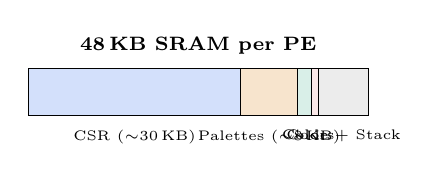
\begin{tikzpicture}[xscale=0.09, yscale=0.6]
  % Total bar
  \fill[cpuBlue!20]   (0,0) rectangle (30,1);  % CSR
  \fill[warnOrange!20] (30,0) rectangle (38,1); % palette
  \fill[confirmGreen!15](38,0) rectangle (40,1); % color array
  \fill[conflictRed!10](40,0) rectangle (41,1);  % flags
  \fill[gray!15]       (41,0) rectangle (48,1);  % code+stack

  \draw (0,0) rectangle (48,1);
  \draw (30,0)--(30,1); \draw (38,0)--(38,1);
  \draw (40,0)--(40,1); \draw (41,0)--(41,1);

  \node[font=\tiny,anchor=north] at (15,-0.1) {CSR (${\sim}$30\,KB)};
  \node[font=\tiny,anchor=north] at (34,-0.1) {Palettes (${\sim}$8\,KB)};
  \node[font=\tiny,anchor=north] at (39.5,-0.1) {\rotatebox{0}{Colors}};
  \node[font=\tiny,anchor=north] at (44.5,-0.1) {Code + Stack};

  \node[font=\scriptsize,anchor=south] at (24,1.1) {\textbf{48\,KB SRAM per PE}};
\end{tikzpicture}
\end{center}

\begin{center}
\renewcommand{\arraystretch}{1.2}
\begin{tabular}{lr}
\toprule
\textbf{Component} & \textbf{Approximate Size} \\
\midrule
CSR offsets + adj & ${\sim}$30\,KB (for ${\sim}$500 vertices, degree ${\sim}$30) \\
Palette / color lists & ${\sim}$8\,KB \\
Color array & ${\sim}$2\,KB \\
Conflict flags & ${\sim}$1\,KB \\
Code + stack & ${\sim}$7\,KB \\
\midrule
\textbf{Total} & $\leq$ \textbf{48\,KB} \\
\bottomrule
\end{tabular}
\end{center}

What if the graph is just too big? The answer is straightforward: \textbf{throw more PEs at it}. With up to 750,000 PEs on the WSE-2, even graphs with millions of vertices can be split into pieces small enough that every PE's share fits comfortably within its 48\,KB.

%======================================================================
\section{Implementation: Checkerboard Routing and Software Relay}
\label{sec:implementation}
%======================================================================

The high-level algorithm from Section~\ref{sec:cerebras} hides a critical engineering challenge: \emph{how do wavelets actually reach their destination?} On the WSE, PEs are arranged in a 2D grid, and wavelet routing through the fabric requires careful configuration of \textbf{fabric colors} (hardware channels) to avoid deadlocks.

\subsection{The Routing Problem}

A wavelet from PE\,0 to PE\,3 must traverse PE\,1 and PE\,2. On the WSE, each PE has a \textbf{router} that can be configured per color: for a given color, incoming wavelets from one direction can be forwarded to another direction and/or delivered to the PE's local task (via RAMP).

The na\"ive approach---use a single color for eastbound traffic where every PE does \texttt{rx=WEST, tx=EAST,RAMP}---fails immediately. If PE\,1 tries to \emph{send} its own eastbound wavelet on the same color that pass-through traffic is using, the WSE hardware deadlocks: the PE cannot simultaneously inject a wavelet and receive a pass-through wavelet on the same color.

\subsection{Checkerboard Routing}

The solution is \textbf{checkerboard parity}: alternate send/receive colors based on PE position so that no PE ever sends and receives on the same color simultaneously.

We use \textbf{4 fabric colors} for east/west communication (colors 0--3):
\begin{itemize}[nosep]
  \item \textbf{Even-parity PEs} ($(row + col) \bmod 2 = 0$): send east on color\,0, receive from east on color\,2.
  \item \textbf{Odd-parity PEs} ($(row + col) \bmod 2 = 1$): send east on color\,1, receive from east on color\,3.
\end{itemize}

Each wavelet travels \textbf{exactly one hop} per fabric color switch. When PE\,0 (even) sends a wavelet east on color\,0, PE\,1 (odd) receives it via the RAMP. PE\,1's software then re-injects the wavelet eastward on color\,1 (its own send color), and PE\,2 (even) picks it up. This process repeats until the wavelet reaches its destination.

\begin{center}
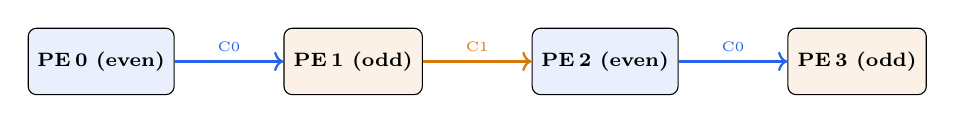
\begin{tikzpicture}[
    pe/.style={draw, rounded corners=3pt, minimum width=50pt, minimum height=24pt, font=\scriptsize\bfseries},
    xscale=1.0
  ]
  \node[pe, fill=cpuBlue!10]  (p0) at (0,0)   {PE\,0 (even)};
  \node[pe, fill=warnOrange!10] (p1) at (3.2,0) {PE\,1 (odd)};
  \node[pe, fill=cpuBlue!10]  (p2) at (6.4,0) {PE\,2 (even)};
  \node[pe, fill=warnOrange!10] (p3) at (9.6,0) {PE\,3 (odd)};

  \draw[->,thick,cpuBlue] (p0.east) -- node[above,font=\tiny] {C0} (p1.west);
  \draw[->,thick,warnOrange] (p1.east) -- node[above,font=\tiny] {C1} (p2.west);
  \draw[->,thick,cpuBlue] (p2.east) -- node[above,font=\tiny] {C0} (p3.west);
\end{tikzpicture}
\end{center}

Route configurations per PE color (eastbound example):
\begin{center}
\renewcommand{\arraystretch}{1.2}
\begin{tabular}{llll}
\toprule
\textbf{Parity} & \textbf{Color} & \textbf{rx} & \textbf{tx} \\
\midrule
Even & C0 (send east) & RAMP & EAST \\
Even & C1 (recv east) & WEST & RAMP \\
Odd  & C0 (recv east) & WEST & RAMP \\
Odd  & C1 (send east) & RAMP & EAST \\
\bottomrule
\end{tabular}
\end{center}

\subsection{Software Relay Buffers}

Since each wavelet only travels one hop at a time, intermediate PEs must \textbf{relay} wavelets that are not destined for them. Each PE maintains per-direction \textbf{circular relay queues}:

\begin{lstlisting}
relay_east_q[max_relay]   // circular buffer for eastbound relay
relay_west_q[max_relay]   // circular buffer for westbound relay
\end{lstlisting}

When a PE receives a wavelet, it inspects the packed \texttt{dest\_pe} field:
\begin{itemize}[nosep]
  \item If \texttt{dest\_pe == my\_pe}: process immediately (update neighbor color table).
  \item If \texttt{dest\_pe > my\_pe}: push onto \texttt{relay\_east\_q} (forward east).
  \item If \texttt{dest\_pe < my\_pe}: push onto \texttt{relay\_west\_q} (forward west).
\end{itemize}

\paragraph{Drain rate.} Relay wavelets are drained \textbf{one per task activation}. The send task alternates between sending the PE's own boundary wavelets and draining one relay entry. This ``cooperative scheduling'' between send and relay prevents output FIFO deadlock: between every send, receive data tasks can fire, keeping the pipeline fluid.

\subsection{Wavelet Encoding}

Each wavelet is a single 32-bit word, packed as follows:
\begin{center}
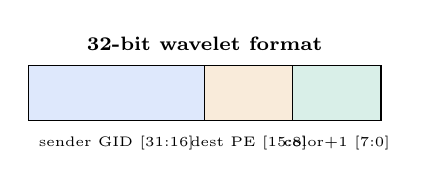
\begin{tikzpicture}[xscale=0.14, yscale=0.7]
  \fill[cpuBlue!15] (0,0) rectangle (16,1);
  \fill[warnOrange!15] (16,0) rectangle (24,1);
  \fill[confirmGreen!15] (24,0) rectangle (32,1);
  \draw (0,0) rectangle (32,1);
  \draw (16,0)--(16,1); \draw (24,0)--(24,1);

  \node[font=\tiny,anchor=north] at (8,-0.1) {sender GID [31:16]};
  \node[font=\tiny,anchor=north] at (20,-0.1) {dest PE [15:8]};
  \node[font=\tiny,anchor=north] at (28,-0.1) {color+1 [7:0]};

  \node[font=\scriptsize,anchor=south] at (16,1.1) {\textbf{32-bit wavelet format}};
\end{tikzpicture}
\end{center}

\begin{itemize}[nosep]
  \item \textbf{Bits [31:16]}: Sender's global vertex ID (supports up to 65,535 vertices).
  \item \textbf{Bits [15:8]}: Destination PE index (supports up to 255 PEs in 1D).
  \item \textbf{Bits [7:0]}: Assigned color $+ 1$ (0 reserved, supports palette up to 255).
\end{itemize}

The destination PE is computed from the neighbor's global vertex ID using the partition chunk size: $\texttt{dest\_pe} = \min(\lfloor \texttt{gid} / \texttt{chunk} \rfloor,\; P{-}1)$.

\subsection{Count-Based Completion Detection}

A key insight eliminates the need for ``done'' sentinel wavelets. The host \textbf{precomputes} the exact number of data wavelets each PE will receive per round:

\[
  \texttt{expected\_total\_recv}[p] = \sum_{\substack{q \neq p}} \bigl|\{(u,v) \in \text{boundary}(q) : \texttt{gid\_to\_pe}(v) = p\}\bigr|
\]

Each PE's receive handler decrements a counter \texttt{recv\_remaining}. When it reaches zero, all data wavelets have arrived. Combined with the send-completion flag and relay-drained check, this precisely determines when the data exchange phase is complete---without any extra sentinel traffic.

%======================================================================
\section{Implementation: Sync Barrier Protocol}
\label{sec:sync-impl}
%======================================================================

In 1D mode, a \textbf{software-implemented sync barrier} using 3 additional fabric colors (C8, C9, C10) ensures BSP semantics. The barrier has two phases:

\subsection{Phase 1: OR-Reduce (East $\to$ West)}

After all data wavelets are sent and received, the \textbf{eastmost PE} initiates a reduce chain:

\begin{enumerate}[nosep]
  \item PE$_{N-1}$ (east edge) sends a sync wavelet westward containing its \texttt{has\_uncolored} flag.
  \item Each interior PE receives the sync wavelet from its east neighbor, OR-combines it with its own \texttt{has\_uncolored} flag, and forwards the result westward.
  \item PE$_0$ (west edge) receives the fully reduced value.
\end{enumerate}

The reduce uses \textbf{alternating colors} (C8/C9) by PE parity to avoid same-color send/recv collision, identical to the checkerboard pattern for data.

\subsection{Phase 2: Broadcast (West $\to$ East)}

PE$_0$ sends the reduced \texttt{has\_uncolored} flag eastward on color C10:

\begin{enumerate}[nosep]
  \item PE$_0$ sends broadcast wavelet east.
  \item Each interior PE receives from the west, forwards east, and delivers to its local task.
  \item PE$_{N-1}$ receives and delivers locally.
\end{enumerate}

Color C10 uses \texttt{rx=WEST, tx=\{EAST, RAMP\}} on interior PEs, which is safe because no PE injects its own wavelet on C10 (only PE$_0$ originates).

\subsection{Two-Flag Gate: \texttt{maybe\_proceed()}}

Each PE tracks two flags:
\begin{itemize}[nosep]
  \item \texttt{local\_data\_done}: set when all expected data wavelets received.
  \item \texttt{sync\_barrier\_done}: set when broadcast received (or sent, for PE$_0$).
\end{itemize}

Only when \textbf{both} flags are true does the PE proceed to \texttt{detect\_resolve}. This ensures no PE inspects boundary colors before every other PE has finished sending. If the reduced \texttt{has\_uncolored} flag is zero (all vertices globally colored), the PE skips detection and exits immediately.

\begin{center}
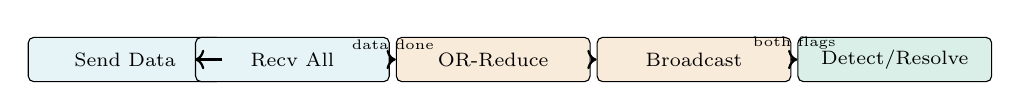
\begin{tikzpicture}[
    box/.style={draw, rounded corners=2pt, minimum height=16pt, font=\scriptsize, fill=wseColor!10, minimum width=70pt},
    arr/.style={->,thick},
    xscale=0.85
  ]
  \node[box] (send) at (0,0) {Send Data};
  \node[box] (recv) at (2.5,0) {Recv All};
  \node[box, fill=warnOrange!15] (reduce) at (5.5,0) {OR-Reduce};
  \node[box, fill=warnOrange!15] (bcast) at (8.5,0) {Broadcast};
  \node[box, fill=confirmGreen!15] (detect) at (11.5,0) {Detect/Resolve};

  \draw[arr] (send)--(recv);
  \draw[arr] (recv)--(reduce) node[midway,above,font=\tiny] {data done};
  \draw[arr] (reduce)--(bcast);
  \draw[arr] (bcast)--(detect) node[midway,above,font=\tiny] {both flags};
\end{tikzpicture}
\end{center}

%======================================================================
\section{Implementation: Task Chaining and BSP Loop}
\label{sec:task-chain}
%======================================================================

The entire BSP round loop runs autonomously on the fabric with \textbf{zero host intervention} between rounds. The host only loads graph data, calls \texttt{start\_coloring()}, waits for completion, and reads back the result.

\subsection{Task Chain Within One Round}

Each round follows this task chain:

\begin{enumerate}[nosep]
  \item \textbf{\texttt{speculate}}: Pick tentative colors for all uncolored vertices. Resolve intra-PE conflicts (higher GID yields). Activate \texttt{send\_boundary}.
  \item \textbf{\texttt{send\_boundary}}: Sort boundary wavelets into per-direction buffers. Open receive window (\texttt{unblock\_all\_recv}). Activate \texttt{send\_wavelet}.
  \item \textbf{\texttt{send\_wavelet}}: Send one wavelet per activation (own data or relay drain). Interleaves with \texttt{recv\_*} data tasks automatically. Reaches phase 4 (done) and calls \texttt{check\_completion}.
  \item \textbf{\texttt{check\_completion}}: When all own data sent, all expected wavelets received, and all relay buffers drained $\to$ triggers \texttt{on\_data\_complete()}.
  \item \textbf{\texttt{on\_data\_complete}}: Initiates sync barrier (OR-reduce chain).
  \item \textbf{Sync barrier}: \texttt{sync\_reduce\_recv} $\to$ \texttt{sync\_bcast\_recv} $\to$ \texttt{maybe\_proceed()}.
  \item \textbf{\texttt{detect\_resolve}}: Check boundary conflicts, resolve (higher GID yields), reset state, activate \texttt{speculate} for a new round.
\end{enumerate}

\subsection{Termination}

The sync barrier's OR-reduced flag tells every PE whether any vertex globally remains uncolored. If the flag is zero after at least one round, \texttt{maybe\_proceed()} activates the \texttt{exit\_task} directly, which stops the hardware cycle counter and unblocks the host command stream.

%======================================================================
\section{Experimental Results}
\label{sec:results}
%======================================================================

We validated the implementation on the Cerebras SDK simulator across 8~test inputs derived from Pauli commutativity graphs, with PE counts from 4 to 16. Table~\ref{tab:results} summarizes representative results.

\begin{table}[h]
\centering
\caption{Coloring results on the Cerebras simulator (1D layout, checkerboard routing).}
\label{tab:results}
\renewcommand{\arraystretch}{1.15}
\begin{tabular}{lrrrr}
\toprule
\textbf{Test Input} & \textbf{Nodes} & \textbf{PEs} & \textbf{Colors} & \textbf{Cycles} \\
\midrule
test1\_all\_commute  & 4  & 4  & 3 & 13{,}155 \\
test2\_triangle      & 4  & 4  & 2 & 7{,}570 \\
test3\_3pairs        & 6  & 4  & 3 & 43{,}164 \\
test3\_3pairs        & 6  & 6  & 3 & 22{,}673 \\
test5\_dense         & 8  & 4  & 3 & 39{,}638 \\
test5\_dense         & 8  & 8  & 3 & 22{,}180 \\
test6\_12nodes       & 12 & 4  & 5 & 219{,}199 \\
test6\_12nodes       & 12 & 8  & 5 & 143{,}840 \\
test6\_12nodes       & 12 & 12 & 6 & 112{,}710 \\
test7\_complete\_K16 & 16 & 4  & 6 & 331{,}696 \\
test7\_complete\_K16 & 16 & 8  & 7 & 191{,}841 \\
test7\_complete\_K16 & 16 & 16 & 6 & 135{,}723 \\
test8\_structured    & 10 & 4  & 6 & 87{,}357 \\
test8\_structured    & 10 & 8  & 6 & 79{,}098 \\
test8\_structured    & 10 & 10 & 6 & 88{,}435 \\
\bottomrule
\end{tabular}
\end{table}

\noindent\textbf{Key observations:}
\begin{itemize}[nosep]
  \item \textbf{All 41 eligible configurations passed} with correct colorings (zero conflicts, all vertices colored).
  \item \textbf{Non-power-of-2 PE counts} (5, 6, 7, 9, 10, 11, 13, 14, 15) all work correctly, validating the division-free routing.
  \item \textbf{Scaling:} Doubling PEs roughly halves cycle count for larger graphs (e.g., K16 at 4 PEs: 331K cycles $\to$ 16 PEs: 136K cycles, a $2.4\times$ speedup).
  \item \textbf{Color quality:} Number of colors used matches or is close to the chromatic number. Small variations across PE counts arise from partition-dependent conflict patterns.
\end{itemize}

\end{document}
